\documentclass[aspectratio=169]{beamer}

% Theme
\usetheme{default}
\usecolortheme{beaver}

% Packages
\usepackage{amsmath,amssymb,amsthm}
\usepackage{mathtools}
\usepackage{bm}
\usepackage{tikz}
\usetikzlibrary{arrows.meta,positioning,calc,decorations.markings}

% Custom commands
\newcommand{\R}{\mathbb{R}}
\newcommand{\Ld}{\mathcal{L}^d}
\newcommand{\Pp}{\mathcal{P}_p}

% Title
\title{Introduction to Optimal Transport}
\subtitle{From Monge to Kantorovich}
\author{}
\date{}

\begin{document}

%==============================================================================
\begin{frame}
\titlepage
\end{frame}

%==============================================================================
\begin{frame}{Outline}
\tableofcontents[hideallsubsections]
\end{frame}

%==============================================================================
\section{The Monge Problem}
%==============================================================================

\begin{frame}{The Monge Problem (1781)}
Given two densities $f, g \geq 0$ on $\R^d$ with $\int f(x)\,dx = \int g(y)\,dy = 1$,\\
find a map $T: \R^d \to \R^d$ such that:
\[
\int_A g(y)\,dy = \int_{T^{-1}(A)} f(x)\,dx \quad \text{for any Borel set } A \subset \R^d
\]
minimizing the \textbf{total cost}:
\[
M(T) := \int_{\R^d} \underbrace{|T(x) - x|}_{\text{distance}} \cdot \underbrace{f(x)}_{\text{density}} \, dx
\]

\vspace{0.3cm}
\begin{center}
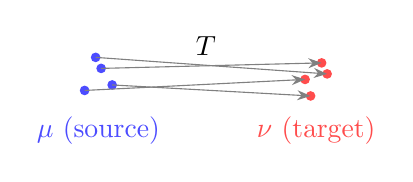
\begin{tikzpicture}[scale=0.7]
    \foreach \x/\y in {0/0, 0.3/0.4, 0.5/0.1, 0.2/0.6} {
        \fill[blue!70] (\x,\y) circle (2.5pt);
    }
    \node[below,blue!70] at (0.25,-0.3) {$\mu$ (source)};

    \foreach \x/\y in {4/0.2, 4.3/0.5, 4.1/-0.1, 4.4/0.3} {
        \fill[red!70] (\x,\y) circle (2.5pt);
    }
    \node[below,red!70] at (4.2,-0.3) {$\nu$ (target)};

    \draw[-{Stealth},gray] (0.5,0.1) -- (4.1,-0.1);
    \draw[-{Stealth},gray] (0.3,0.4) -- (4.3,0.5);
    \draw[-{Stealth},gray] (0,0) -- (4,0.2);
    \draw[-{Stealth},gray] (0.2,0.6) -- (4.4,0.3);

    \node at (2.2,0.8) {$T$};
\end{tikzpicture}
\end{center}
\end{frame}

%==============================================================================
\begin{frame}{Push-forward Measure}
For a measure $\mu$ on $X$ and a map $T: X \to Y$, the \textbf{push-forward} $T_\#\mu$ is:
\[
(T_\#\mu)(A) = \mu(T^{-1}(A)) \quad \text{for every measurable } A \subset Y
\]
Equivalently:
\[
\int_Y \phi(y) \, d(T_\#\mu)(y) = \int_X \underbrace{\phi(T(x))}_{\text{composition}} \, d\mu(x)
\]
for every measurable $\phi$.

\vspace{0.3cm}
\begin{center}
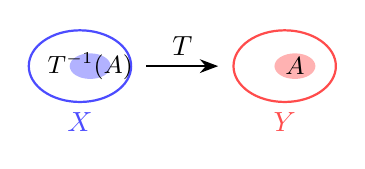
\begin{tikzpicture}[scale=0.65]
    \draw[blue!70,thick] (0,0) ellipse (1 and 0.7);
    \node[blue!70] at (0,-1.1) {$X$};
    \fill[blue!30] (0.2,0) ellipse (0.4 and 0.25);
    \node[font=\small] at (0.2,0) {$T^{-1}(A)$};

    \draw[-{Stealth},thick] (1.3,0) -- node[above] {$T$} (2.7,0);

    \draw[red!70,thick] (4,0) ellipse (1 and 0.7);
    \node[red!70] at (4,-1.1) {$Y$};
    \fill[red!30] (4.2,0) ellipse (0.4 and 0.25);
    \node[font=\small] at (4.2,0) {$A$};
\end{tikzpicture}
\end{center}
\end{frame}

%==============================================================================
\begin{frame}{Exercise 1: Push-forward Computation}
\textbf{Problem:} Let $\mu$ be the uniform measure on $[0,1]$ (i.e., $d\mu = dx$).\\
Let $T(x) = 2x$.

\vspace{0.5cm}
\begin{enumerate}
    \item[(a)] Find the push-forward measure $\nu = T_\#\mu$.
    \item[(b)] Verify using the formula: $\int_{\R} \phi(y)\,d\nu(y) = \int_0^1 \phi(T(x))\,dx$
\end{enumerate}

\vspace{0.5cm}
\textit{Hint:} What is the support of $\nu$? What is its density?
\end{frame}

%==============================================================================
\begin{frame}{Solution 1}
\begin{columns}
\begin{column}{0.55\textwidth}
\textbf{(a)} The map $T(x) = 2x$ sends $[0,1]$ to $[0,2]$.

For the density, use the Jacobian formula:
\[
g(T(x)) \cdot |T'(x)| = f(x) \quad \Rightarrow \quad g(2x) \cdot 2 = 1
\]
So $g(y) = \frac{1}{2}$ on $[0,2]$.

\vspace{0.2cm}
\textbf{Answer:} $\nu = T_\#\mu$ is uniform on $[0,2]$ with density $g(y) = \frac{1}{2}$.

\vspace{0.3cm}
\textbf{(b)} Verification:
\[
\int_0^2 \phi(y) \cdot \frac{1}{2}\,dy = \int_0^1 \phi(2x)\,dx \;\checkmark
\]
\end{column}
\begin{column}{0.45\textwidth}
\begin{center}
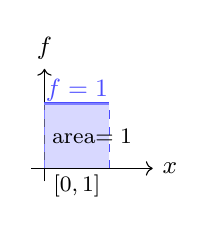
\begin{tikzpicture}[scale=0.55]
    % Source density f=1 on [0,1]
    \draw[->] (-0.3,0) -- (2.5,0) node[right] {\small $x$};
    \draw[->] (0,-0.3) -- (0,2.3) node[above] {\small $f$};
    \draw[blue!70, very thick] (0,1.5) -- (1.5,1.5);
    \draw[blue!70, dashed] (0,0) -- (0,1.5);
    \draw[blue!70, dashed] (1.5,0) -- (1.5,1.5);
    \fill[blue!30, opacity=0.5] (0,0) rectangle (1.5,1.5);
    \node[blue!70, font=\small] at (0.75,1.8) {$f=1$};
    \node[font=\footnotesize] at (0.75,-0.4) {$[0,1]$};
    \node at (1.1,0.75) {\footnotesize area$=1$};
\end{tikzpicture}

\vspace{0.1cm}
$\downarrow$ \small $T(x)=2x$ stretches

\vspace{0.1cm}
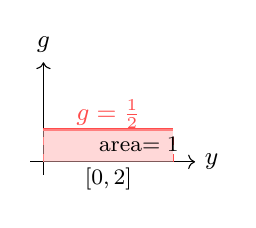
\begin{tikzpicture}[scale=0.55]
    % Target density g=1/2 on [0,2]
    \draw[->] (-0.3,0) -- (3.5,0) node[right] {\small $y$};
    \draw[->] (0,-0.3) -- (0,2.3) node[above] {\small $g$};
    \draw[red!70, very thick] (0,0.75) -- (3,0.75);
    \draw[red!70, dashed] (0,0) -- (0,0.75);
    \draw[red!70, dashed] (3,0) -- (3,0.75);
    \fill[red!30, opacity=0.5] (0,0) rectangle (3,0.75);
    \node[red!70, font=\small] at (1.5,1.1) {$g=\frac{1}{2}$};
    \node[font=\footnotesize] at (1.5,-0.4) {$[0,2]$};
    \node at (2.2,0.4) {\footnotesize area$=1$};
\end{tikzpicture}
\end{center}
\end{column}
\end{columns}
\end{frame}

%==============================================================================
\begin{frame}{General Monge Problem}
For a general cost function $c: X \times Y \to \R$:
\[
\text{(MP)} \quad \min \left\{ M(T) := \int_X \underbrace{c(x, T(x))}_{\text{cost to move } x \to T(x)} \, d\mu(x) \;:\; T_\#\mu = \nu \right\}
\]

\vspace{0.3cm}
If $\mu, \nu$ have densities $f, g$ and $T$ is smooth, injective:
\[
\underbrace{g(T(x))}_{\text{target density}} \cdot \underbrace{\det(DT(x))}_{\text{volume change}} = \underbrace{f(x)}_{\text{source density}}
\]

\vspace{0.3cm}
\textbf{Common costs:}
\begin{itemize}
    \item $c(x,y) = |x-y|$ \quad (Monge's original)
    \item $c(x,y) = |x-y|^2$ \quad (quadratic/kinetic energy)
\end{itemize}
\end{frame}

%==============================================================================
\begin{frame}{Difficulties with the Monge Problem}
\textbf{Key issue:} A map $T$ cannot split mass!

\vspace{0.3cm}
\begin{center}
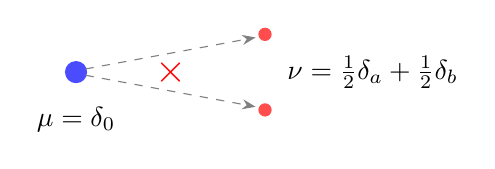
\begin{tikzpicture}[scale=0.8]
    \fill[blue!70] (0,0) circle (5pt);
    \node[below] at (0,-0.4) {$\mu = \delta_0$};

    \fill[red!70] (3,0.6) circle (3pt);
    \fill[red!70] (3,-0.6) circle (3pt);
    \node[right] at (3.2,0) {$\nu = \tfrac{1}{2}\delta_a + \tfrac{1}{2}\delta_b$};

    \draw[-{Stealth},gray,dashed] (0.15,0.05) -- (2.85,0.55);
    \draw[-{Stealth},gray,dashed] (0.15,-0.05) -- (2.85,-0.55);

    \node[red] at (1.5,0) {\Large $\times$};
\end{tikzpicture}
\end{center}

\vspace{0.2cm}
\textbf{Problems:}
\begin{itemize}
    \item Constraint $T_\#\mu = \nu$ is \textbf{nonlinear}
    \item Optimal map may \textbf{not exist}
    \item Weak convergence $T_n \rightharpoonup T$ does not imply $(T_n)_\#\mu \to T_\#\mu$
\end{itemize}

\vspace{0.2cm}
$\Rightarrow$ Problem remained unsolved for $\sim$160 years!
\end{frame}

%==============================================================================
\section{Kantorovich Relaxation}
%==============================================================================

\begin{frame}{Kantorovich's Relaxation (1942)}
\textbf{Key idea:} Replace transport \emph{maps} with transport \emph{plans}.

\vspace{0.3cm}
A \textbf{transport plan} $\gamma$ on $X \times Y$ satisfies:
\[
\underbrace{(\pi_x)_\#\gamma = \mu}_{\text{first marginal}} \quad \text{and} \quad \underbrace{(\pi_y)_\#\gamma = \nu}_{\text{second marginal}}
\]
Denote the set of all such plans by $\Pi(\mu, \nu)$.

\vspace{0.3cm}
\textbf{Kantorovich Problem:}
\[
\text{(KP)} \quad \min_{\gamma \in \Pi(\mu,\nu)} \int_{X \times Y} c(x,y) \, d\gamma(x,y)
\]

\vspace{0.3cm}
\textbf{Advantages:}
\begin{itemize}
    \item Linear objective + linear constraints $\Rightarrow$ \textbf{Linear Programming}
    \item Existence guaranteed (weak-* compactness)
    \item Mass splitting allowed!
\end{itemize}
\end{frame}

%==============================================================================
\begin{frame}{Transport Plan Visualization}
\begin{columns}
\begin{column}{0.5\textwidth}
\textbf{Monge map:}\\
$x \mapsto T(x)$ (one destination)

\vspace{0.5cm}
\textbf{Kantorovich plan:}\\
$\gamma(x,y)$ = mass from $x$ to $y$\\
(can split!)

\vspace{0.5cm}
If $T$ is a Monge map:
\[
\gamma = (\text{Id} \times T)_\#\mu
\]
is a valid plan.
\end{column}
\begin{column}{0.5\textwidth}
\begin{center}
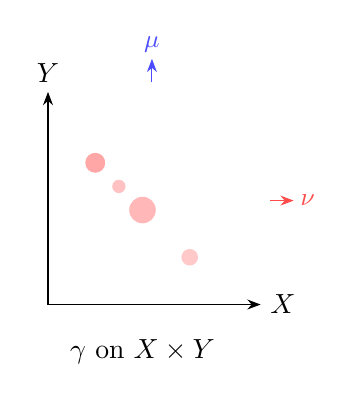
\begin{tikzpicture}[scale=0.6]
    \draw[-{Stealth}] (0,0) -- (4.5,0) node[right] {$X$};
    \draw[-{Stealth}] (0,0) -- (0,4.5) node[above] {$Y$};

    \fill[red!50,opacity=0.7] (1,3) circle (6pt);
    \fill[red!40,opacity=0.7] (2,2) circle (8pt);
    \fill[red!30,opacity=0.7] (3,1) circle (5pt);
    \fill[red!35,opacity=0.7] (1.5,2.5) circle (4pt);

    \node at (2,-1) {$\gamma$ on $X \times Y$};

    \draw[-{Stealth},blue!70] (2.2,4.7) -- (2.2,5.2);
    \node[blue!70,font=\small] at (2.2,5.5) {$\mu$};

    \draw[-{Stealth},red!70] (4.7,2.2) -- (5.2,2.2);
    \node[red!70,font=\small] at (5.5,2.2) {$\nu$};
\end{tikzpicture}
\end{center}
\end{column}
\end{columns}
\end{frame}

%==============================================================================
\begin{frame}{Exercise 2: Discrete Optimal Transport}
\textbf{Problem:} Consider discrete measures on $\{1, 2\}$:
\[
\mu = \frac{1}{2}\delta_1 + \frac{1}{2}\delta_2, \quad \nu = \frac{1}{2}\delta_1 + \frac{1}{2}\delta_2
\]
with cost $c(x,y) = |x-y|^2$.

\vspace{0.3cm}
A transport plan is a $2 \times 2$ matrix $\gamma = \begin{pmatrix} \gamma_{11} & \gamma_{12} \\ \gamma_{21} & \gamma_{22} \end{pmatrix}$ with:
\begin{itemize}
    \item Row sums = $\mu$: $\gamma_{11} + \gamma_{12} = \frac{1}{2}$, $\gamma_{21} + \gamma_{22} = \frac{1}{2}$
    \item Column sums = $\nu$: $\gamma_{11} + \gamma_{21} = \frac{1}{2}$, $\gamma_{12} + \gamma_{22} = \frac{1}{2}$
\end{itemize}

\vspace{0.3cm}
\textbf{Find:} The optimal transport plan minimizing $\sum_{i,j} c(i,j)\gamma_{ij}$.
\end{frame}

%==============================================================================
\begin{frame}{Solution 2}
\begin{columns}
\begin{column}{0.55\textwidth}
Cost matrix: $C = \begin{pmatrix} 0 & 1 \\ 1 & 0 \end{pmatrix}$

\vspace{0.2cm}
Total cost: $\text{Cost}(\gamma) = \gamma_{12} + \gamma_{21}$

\vspace{0.2cm}
From constraints: $\gamma_{12} = \gamma_{21} = \frac{1}{2} - \gamma_{11}$

So: $\text{Cost} = 1 - 2\gamma_{11}$, minimized at $\gamma_{11} = \frac{1}{2}$.

\vspace{0.2cm}
\textbf{Optimal plan:}
\[
\gamma^* = \begin{pmatrix} 1/2 & 0 \\ 0 & 1/2 \end{pmatrix}
\]
$\Rightarrow W_2^2(\mu,\nu) = 0$ (identity map!)
\end{column}
\begin{column}{0.45\textwidth}
\begin{center}
\textbf{Transport Visualization}

\vspace{0.2cm}
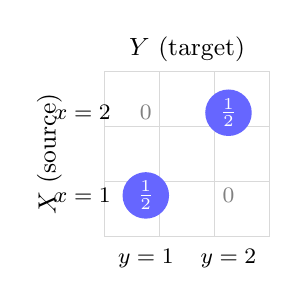
\begin{tikzpicture}[scale=0.7]
    % Grid
    \draw[gray!30] (0,0) grid (3,3);

    % Axes labels
    \node[font=\footnotesize] at (-0.4, 0.75) {$x=1$};
    \node[font=\footnotesize] at (-0.4, 2.25) {$x=2$};
    \node[font=\footnotesize] at (0.75, -0.4) {$y=1$};
    \node[font=\footnotesize] at (2.25, -0.4) {$y=2$};

    % Optimal transport (diagonal)
    \fill[blue!60] (0.75, 0.75) circle (12pt);
    \node[white, font=\footnotesize\bfseries] at (0.75, 0.75) {$\frac{1}{2}$};
    \fill[blue!60] (2.25, 2.25) circle (12pt);
    \node[white, font=\footnotesize\bfseries] at (2.25, 2.25) {$\frac{1}{2}$};

    % Zero off-diagonal
    \node[gray, font=\footnotesize] at (2.25, 0.75) {$0$};
    \node[gray, font=\footnotesize] at (0.75, 2.25) {$0$};

    % Axis titles
    \node at (1.5, 3.4) {\small $Y$ (target)};
    \node[rotate=90] at (-1, 1.5) {\small $X$ (source)};
\end{tikzpicture}

\vspace{0.2cm}
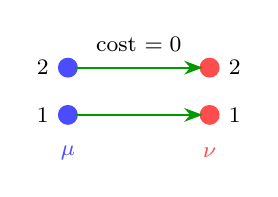
\begin{tikzpicture}[scale=0.6]
    % Source points
    \fill[blue!70] (0, 0.5) circle (6pt);
    \node[left, font=\footnotesize] at (-0.2, 0.5) {$1$};
    \fill[blue!70] (0, 1.5) circle (6pt);
    \node[left, font=\footnotesize] at (-0.2, 1.5) {$2$};
    \node[blue!70, font=\footnotesize] at (0, -0.3) {$\mu$};

    % Target points
    \fill[red!70] (3, 0.5) circle (6pt);
    \node[right, font=\footnotesize] at (3.2, 0.5) {$1$};
    \fill[red!70] (3, 1.5) circle (6pt);
    \node[right, font=\footnotesize] at (3.2, 1.5) {$2$};
    \node[red!70, font=\footnotesize] at (3, -0.3) {$\nu$};

    % Optimal arrows (stay in place)
    \draw[-{Stealth}, thick, green!60!black] (0.15, 0.5) -- (2.85, 0.5);
    \draw[-{Stealth}, thick, green!60!black] (0.15, 1.5) -- (2.85, 1.5);

    \node[font=\footnotesize] at (1.5, 2) {cost $= 0$};
\end{tikzpicture}
\end{center}
\end{column}
\end{columns}
\end{frame}

%==============================================================================
\section{Brenier's Theorem}
%==============================================================================

\begin{frame}{Brenier's Theorem (1991)}
For the \textbf{quadratic cost} $c(x,y) = |x-y|^2$:

\vspace{0.3cm}
\textbf{Theorem (Brenier):} If $\mu \ll \Ld$ (absolutely continuous), then:
\begin{enumerate}
    \item There exists a \textbf{unique} optimal transport map $T$
    \item $T = \nabla u$ for some \textbf{convex function} $u: \R^d \to \R$
\end{enumerate}

\vspace{0.3cm}
\begin{center}
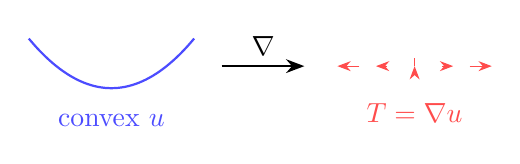
\begin{tikzpicture}[scale=0.7]
    \draw[thick,blue!70] plot[smooth,domain=-1.5:1.5] (\x,{0.4*\x*\x});
    \node[below,blue!70] at (0,-0.3) {convex $u$};

    \draw[-{Stealth},thick] (2,0.4) -- node[above] {$\nabla$} (3.5,0.4);

    \begin{scope}[shift={(5.5,0.4)}]
        \foreach \x in {-1,-0.5,0,0.5,1} {
            \draw[-{Stealth},red!70] (\x,0) -- ({\x+0.4*\x},0);
        }
        \node[below,red!70] at (0,-0.5) {$T = \nabla u$};
    \end{scope}
\end{tikzpicture}
\end{center}

\vspace{0.2cm}
The optimal transport is the \textbf{gradient of a convex function}.
\end{frame}

%==============================================================================
\begin{frame}{Monge-Amp\`ere Equation}
Combining the Jacobian equation with $T = \nabla u$:
\[
g(\nabla u(x)) \cdot \det(D^2 u(x)) = f(x)
\]
Rearranging:
\[
\det\bigl(\underbrace{D^2 u(x)}_{\text{Hessian}}\bigr) = \frac{f(x)}{g(\nabla u(x))}
\]

\vspace{0.3cm}
This is the \textbf{Monge-Amp\`ere equation}:
\begin{itemize}
    \item Fully nonlinear elliptic PDE
    \item Well-posed in the class of \textbf{convex functions}
    \item Rich regularity theory (Caffarelli, 1990s)
\end{itemize}

\vspace{0.3cm}
\textbf{Polar Factorization:} Any $v: \R^d \to \R^d$ can be written as $v = \nabla u \circ s$ where $u$ is convex and $s$ is measure-preserving.
\end{frame}

%==============================================================================
\begin{frame}{Exercise 3: Brenier Map in 1D}
\textbf{Problem:} Let $\mu = \text{Uniform}[0,1]$ and $\nu = \text{Uniform}[1,3]$.

\vspace{0.3cm}
\begin{enumerate}
    \item[(a)] Find the optimal transport map $T$ for cost $c(x,y) = |x-y|^2$.
    \item[(b)] Find the convex function $u$ such that $T = u'$.
    \item[(c)] Compute $W_2^2(\mu,\nu)$.
\end{enumerate}

\vspace{0.5cm}
\textit{Hint:} In 1D, the optimal map is the \textbf{monotone rearrangement}: it maps the $p$-th quantile of $\mu$ to the $p$-th quantile of $\nu$.
\end{frame}

%==============================================================================
\begin{frame}{Solution 3}
\begin{columns}
\begin{column}{0.5\textwidth}
\textbf{(a)} Quantile functions:
\begin{itemize}
    \item $F_\mu^{-1}(p) = p$ for $p \in [0,1]$
    \item $F_\nu^{-1}(p) = 1 + 2p$ for $p \in [0,1]$
\end{itemize}
Optimal map: $T(x) = 1 + 2x$

\vspace{0.2cm}
\textbf{(b)} Since $T(x) = u'(x)$:
\[
u(x) = x + x^2 + C
\]
(Convex: $u''(x) = 2 > 0$)

\vspace{0.2cm}
\textbf{(c)} $W_2^2(\mu,\nu) = \int_0^1 |1+x|^2\,dx = \frac{7}{3}$
\end{column}
\begin{column}{0.5\textwidth}
\begin{center}
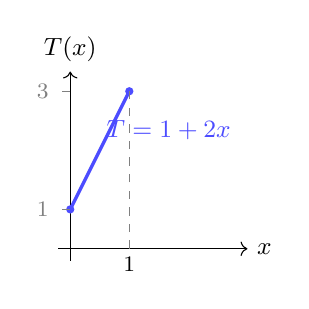
\begin{tikzpicture}[scale=0.5]
    % Optimal map T(x) = 1+2x
    \draw[->] (-0.3,0) -- (4.5,0) node[right] {\small $x$};
    \draw[->] (0,-0.3) -- (0,4.5) node[above] {\small $T(x)$};

    % T(x) = 1 + 2x line
    \draw[blue!70, very thick, domain=0:1.5] plot (\x, {1 + 2*\x});

    % Reference points
    \fill[blue!70] (0, 1) circle (3pt);
    \fill[blue!70] (1.5, 4) circle (3pt);

    % Dashed guides
    \draw[dashed, gray] (0,1) -- (-0.3,1) node[left] {\footnotesize $1$};
    \draw[dashed, gray] (1.5,0) -- (1.5,4);
    \draw[dashed, gray] (0,4) -- (-0.3,4) node[left] {\footnotesize $3$};

    \node[font=\footnotesize] at (1.5, -0.4) {$1$};
    \node[blue!70] at (2.5, 3) {\small $T=1+2x$};
\end{tikzpicture}

\vspace{0.2cm}
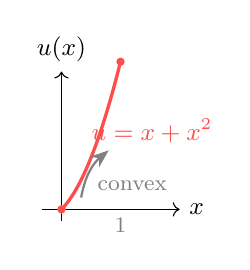
\begin{tikzpicture}[scale=0.5]
    % Convex potential u(x) = x + x^2
    \draw[->] (-0.5,0) -- (3,0) node[right] {\small $x$};
    \draw[->] (0,-0.3) -- (0,3.5) node[above] {\small $u(x)$};

    % u(x) = x + x^2
    \draw[red!70, very thick, domain=0:1.5] plot (\x, {\x + \x*\x});

    \fill[red!70] (0, 0) circle (3pt);
    \fill[red!70] (1.5, 3.75) circle (3pt);

    \node[red!70] at (2.3, 2) {\small $u=x+x^2$};
    \node[font=\footnotesize, gray] at (1.5, -0.4) {$1$};

    % Convexity indicator
    \draw[-{Stealth}, gray, thick] (0.5, 0.3) to[bend left=20] (1.2, 1.5);
    \node[gray, font=\footnotesize] at (1.8, 0.6) {convex};
\end{tikzpicture}

\vspace{0.1cm}
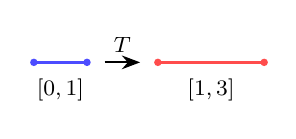
\begin{tikzpicture}[scale=0.45]
    % Visual: [0,1] -> [1,3]
    \draw[blue!70, very thick] (0,0) -- (1.5,0);
    \node[below, font=\footnotesize] at (0.75, -0.2) {$[0,1]$};
    \fill[blue!70] (0,0) circle (3pt);
    \fill[blue!70] (1.5,0) circle (3pt);

    \draw[-{Stealth}, thick] (2,0) -- node[above, font=\footnotesize] {$T$} (3,0);

    \draw[red!70, very thick] (3.5,0) -- (6.5,0);
    \node[below, font=\footnotesize] at (5, -0.2) {$[1,3]$};
    \fill[red!70] (3.5,0) circle (3pt);
    \fill[red!70] (6.5,0) circle (3pt);
\end{tikzpicture}
\end{center}
\end{column}
\end{columns}
\end{frame}

%==============================================================================
\section{Wasserstein Distance}
%==============================================================================

\begin{frame}{Wasserstein Distance}
\textbf{Definition:} For probability measures $\mu, \nu$ and $p \geq 1$:
\[
W_p(\mu, \nu) := \left( \inf_{\gamma \in \Pi(\mu,\nu)} \int_{X \times Y} \underbrace{|x-y|^p}_{\text{cost}} \, d\gamma(x,y) \right)^{1/p}
\]

\vspace{0.3cm}
\textbf{Properties:}
\begin{itemize}
    \item $W_p$ is a \textbf{metric} on $\Pp(\R^d) = \{\mu : \int |x|^p \, d\mu < \infty\}$
    \item Metrizes weak convergence + convergence of $p$-th moments
    \item For $p=2$ (Brenier): $W_2^2(\mu,\nu) = \int |x - \nabla u(x)|^2 \, d\mu$
\end{itemize}

\vspace{0.3cm}
\begin{center}
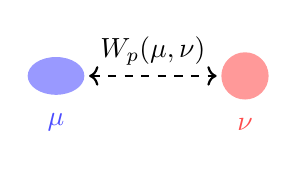
\begin{tikzpicture}[scale=0.6]
    \fill[blue!40] (0,0) ellipse (0.6 and 0.4);
    \node[below,blue!70] at (0,-0.6) {$\mu$};

    \fill[red!40] (4,0) ellipse (0.5 and 0.5);
    \node[below,red!70] at (4,-0.7) {$\nu$};

    \draw[<->,dashed,thick] (0.7,0) -- node[above] {$W_p(\mu,\nu)$} (3.4,0);
\end{tikzpicture}
\end{center}
\end{frame}

%==============================================================================
\begin{frame}{Geodesics in Wasserstein Space}
The \textbf{geodesic} from $\mu_0$ to $\mu_1$ in $(\mathcal{P}_2, W_2)$:
\[
\mu_t = \bigl(\underbrace{(1-t)\text{Id} + t\nabla u}_{\text{linear interpolation of positions}}\bigr)_\# \mu_0, \quad t \in [0,1]
\]
where $\nabla u$ is the optimal map from $\mu_0$ to $\mu_1$.

\vspace{0.3cm}
\begin{center}
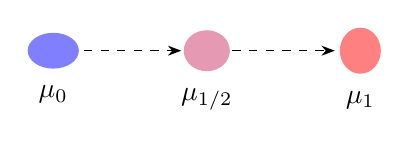
\begin{tikzpicture}[scale=0.65]
    \fill[blue!50] (0,0) ellipse (0.5 and 0.35);
    \node[below] at (0,-0.5) {$\mu_0$};

    \fill[purple!40] (3,0) ellipse (0.45 and 0.4);
    \node[below] at (3,-0.55) {$\mu_{1/2}$};

    \fill[red!50] (6,0) ellipse (0.4 and 0.45);
    \node[below] at (6,-0.6) {$\mu_1$};

    \draw[-{Stealth},dashed] (0.6,0) -- (2.5,0);
    \draw[-{Stealth},dashed] (3.5,0) -- (5.5,0);
\end{tikzpicture}
\end{center}

\vspace{0.2cm}
\textbf{Displacement interpolation:} Particles move along straight lines at constant speed.

\vspace{0.2cm}
\textbf{McCann's Displacement Convexity (1997):}
\[
\mathcal{F}(\mu_t) \leq (1-t)\mathcal{F}(\mu_0) + t\mathcal{F}(\mu_1)
\]
for many functionals $\mathcal{F}$.
\end{frame}

%==============================================================================
\begin{frame}{Exercise 4: $W_1$ Distance (Earth Mover)}
\textbf{Problem:} Compute $W_1(\mu, \nu)$ where:
\[
\mu = \delta_0, \quad \nu = \frac{1}{2}\delta_{-1} + \frac{1}{2}\delta_{1}
\]

\vspace{0.5cm}
\textit{Recall:} $W_1(\mu,\nu) = \inf_{\gamma \in \Pi(\mu,\nu)} \int |x-y| \, d\gamma(x,y)$

\vspace{0.5cm}
\textit{Hint:} Since $\mu = \delta_0$, any transport plan $\gamma$ must have the form:
\[
\gamma = \alpha \cdot \delta_{(0,-1)} + (1-\alpha) \cdot \delta_{(0,1)}
\]
for some $\alpha \in [0,1]$. What constraint does $(\pi_y)_\#\gamma = \nu$ give?
\end{frame}

%==============================================================================
\begin{frame}{Solution 4}
\begin{columns}
\begin{column}{0.5\textwidth}
From $(\pi_y)_\#\gamma = \nu = \frac{1}{2}\delta_{-1} + \frac{1}{2}\delta_1$:
\[
\alpha = \frac{1}{2}, \quad 1-\alpha = \frac{1}{2}
\]

Unique transport plan:
\[
\gamma = \frac{1}{2}\delta_{(0,-1)} + \frac{1}{2}\delta_{(0,1)}
\]

\vspace{0.2cm}
The cost:
\[
W_1 = \frac{1}{2}|0-(-1)| + \frac{1}{2}|0-1| = 1
\]

\vspace{0.2cm}
\textbf{Note:} No Monge solution exists (mass must split), but Kantorovich gives unique optimal plan!
\end{column}
\begin{column}{0.5\textwidth}
\begin{center}
\textbf{Mass Splitting Visualization}

\vspace{0.2cm}
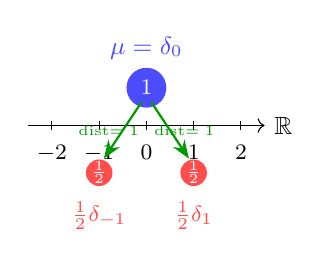
\begin{tikzpicture}[scale=0.6]
    % Number line
    \draw[->] (-2.5,0) -- (2.5,0) node[right] {\small $\R$};

    % Ticks
    \foreach \x in {-2,-1,0,1,2} {
        \draw (\x, 0.1) -- (\x, -0.1);
        \node[below, font=\footnotesize] at (\x, -0.2) {$\x$};
    }

    % Source: delta_0 (big ball)
    \fill[blue!70] (0, 0.8) circle (12pt);
    \node[above, blue!70, font=\small] at (0, 1.2) {$\mu = \delta_0$};
    \node[white, font=\footnotesize\bfseries] at (0, 0.8) {$1$};

    % Target: delta_{-1} and delta_1 (smaller balls)
    \fill[red!70] (-1, -1) circle (8pt);
    \node[below, red!70, font=\footnotesize] at (-1, -1.4) {$\frac{1}{2}\delta_{-1}$};
    \node[white, font=\tiny\bfseries] at (-1, -1) {$\frac{1}{2}$};

    \fill[red!70] (1, -1) circle (8pt);
    \node[below, red!70, font=\footnotesize] at (1, -1.4) {$\frac{1}{2}\delta_1$};
    \node[white, font=\tiny\bfseries] at (1, -1) {$\frac{1}{2}$};

    % Splitting arrows
    \draw[-{Stealth}, thick, green!60!black] (-0.1, 0.5) -- (-0.9, -0.7);
    \draw[-{Stealth}, thick, green!60!black] (0.1, 0.5) -- (0.9, -0.7);

    % Cost labels
    \node[font=\tiny, green!60!black] at (-0.8, -0.1) {dist$=1$};
    \node[font=\tiny, green!60!black] at (0.8, -0.1) {dist$=1$};
\end{tikzpicture}

\vspace{0.3cm}
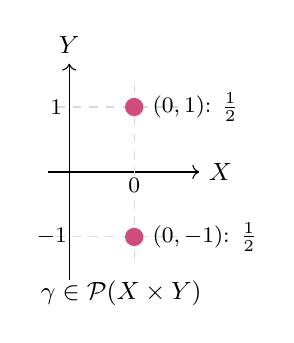
\begin{tikzpicture}[scale=0.55]
    % Transport plan on X x Y
    \draw[->] (-0.5,0) -- (3,0) node[right] {\small $X$};
    \draw[->] (0,-2.5) -- (0,2.5) node[above] {\small $Y$};

    % Grid lines
    \draw[gray!30, dashed] (1.5, -2) -- (1.5, 2);
    \draw[gray!30, dashed] (-0.3, 1.5) -- (2.5, 1.5);
    \draw[gray!30, dashed] (-0.3, -1.5) -- (2.5, -1.5);

    % Points of support
    \fill[purple!70] (1.5, 1.5) circle (6pt);
    \node[right, font=\footnotesize] at (1.7, 1.5) {$(0,1)$: $\frac{1}{2}$};

    \fill[purple!70] (1.5, -1.5) circle (6pt);
    \node[right, font=\footnotesize] at (1.7, -1.5) {$(0,-1)$: $\frac{1}{2}$};

    % Labels
    \node[font=\footnotesize] at (1.5, -0.3) {$0$};
    \node[font=\footnotesize] at (-0.3, 1.5) {$1$};
    \node[font=\footnotesize] at (-0.4, -1.5) {$-1$};

    \node at (1.2, -2.8) {\small $\gamma \in \mathcal{P}(X \times Y)$};
\end{tikzpicture}
\end{center}
\end{column}
\end{columns}
\end{frame}

%==============================================================================
\section{Gradient Flows}
%==============================================================================

\begin{frame}{Gradient Flows in Wasserstein Space}
\begin{columns}
\begin{column}{0.55\textwidth}
\textbf{Key insight:} Many PDEs are gradient flows in $(\mathcal{P}_2, W_2)$.

\vspace{0.2cm}
\textbf{Gradient flow} of functional $\mathcal{F}$:
\[
\partial_t \rho = -\text{grad}_{W_2} \mathcal{F}(\rho)
\]

\vspace{0.2cm}
\textbf{Example: Heat equation}
\[
\partial_t \rho = \Delta \rho
\]
is the gradient flow of the \textbf{entropy}:
\[
\mathcal{F}(\rho) = \int_{\R^d} \underbrace{\rho(x) \log \rho(x)}_{\text{entropy density}} \, dx
\]

\vspace{0.2cm}
\textbf{Other examples:}
\begin{itemize}
    \item Porous medium: $\mathcal{F}(\rho) = \frac{1}{m-1}\int \rho^m$
    \item Fokker-Planck: $\mathcal{F}(\rho) = \int \rho \log \rho + \int V \rho$
\end{itemize}
\end{column}
\begin{column}{0.45\textwidth}
\begin{center}
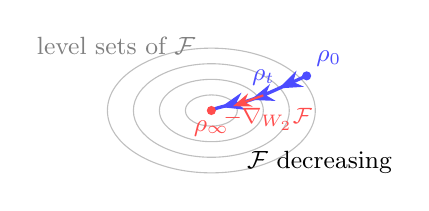
\begin{tikzpicture}[scale=0.55]
    % Energy surface (contour lines)
    \foreach \r in {0.6, 1.2, 1.8, 2.4} {
        \draw[gray!50] (0,0) ellipse ({\r} and {\r*0.6});
    }

    % Gradient flow path
    \draw[blue!70, very thick,
        decoration={markings, mark=at position 0.3 with {\arrow{Stealth}},
                              mark=at position 0.6 with {\arrow{Stealth}},
                              mark=at position 0.9 with {\arrow{Stealth}}},
        postaction={decorate}]
        (2.2, 0.8) .. controls (1.5, 0.5) and (1, 0.2) .. (0.3, 0.1) .. controls (0.1, 0.05) .. (0,0);

    % Points on trajectory
    \fill[blue!70] (2.2, 0.8) circle (3pt) node[above right, font=\small] {$\rho_0$};
    \fill[blue!70] (1.2, 0.35) circle (2.5pt) node[above, font=\small] {$\rho_t$};
    \fill[red!70] (0,0) circle (3pt) node[below, font=\small] {$\rho_\infty$};

    % Labels
    \node at (2.5, -1.2) {\small $\mathcal{F}$ decreasing};
    \node[gray] at (-2.2, 1.5) {\small level sets of $\mathcal{F}$};

    % Gradient arrow
    \draw[-{Stealth}, red!70, thick] (1.2, 0.35) -- (0.5, 0.1);
    \node[red!70, font=\footnotesize] at (1.3, -0.2) {$-\nabla_{W_2}\mathcal{F}$};
\end{tikzpicture}

\vspace{0.3cm}
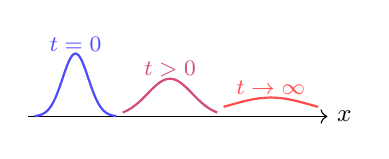
\begin{tikzpicture}[scale=0.4]
    % Time evolution of density
    \draw[->] (-0.5,0) -- (9,0) node[right] {\small $x$};

    % Initial (peaked)
    \draw[blue!70, thick] plot[smooth, domain=-0.3:2.3] (\x, {2*exp(-3*(\x-1)^2)});
    \node[blue!70, font=\footnotesize] at (1, 2.3) {$t=0$};

    % Intermediate
    \draw[purple!70, thick] plot[smooth, domain=2.5:5.5] (\x, {1.2*exp(-1*(\x-4)^2)});
    \node[purple!70, font=\footnotesize] at (4, 1.5) {$t>0$};

    % Final (spread)
    \draw[red!70, thick] plot[smooth, domain=5.7:8.7] (\x, {0.6*exp(-0.3*(\x-7.2)^2)});
    \node[red!70, font=\footnotesize] at (7.2, 0.9) {$t\to\infty$};
\end{tikzpicture}
\end{center}
\end{column}
\end{columns}
\end{frame}

%==============================================================================
\begin{frame}{JKO Scheme}
\begin{columns}
\begin{column}{0.55\textwidth}
\textbf{Jordan-Kinderlehrer-Otto (1998):} Discrete-time approximation.

\vspace{0.2cm}
\[
\rho^{n+1} = \arg\min_\rho \left\{ \underbrace{\frac{1}{2\tau} W_2^2(\rho, \rho^n)}_{\text{stay close to } \rho^n} + \underbrace{\mathcal{F}(\rho)}_{\text{minimize energy}} \right\}
\]

\vspace{0.2cm}
As $\tau \to 0$:
\[
\rho^n \longrightarrow \rho(n\tau) \quad \text{solving } \partial_t \rho = -\text{grad}_{W_2}\mathcal{F}
\]

\vspace{0.3cm}
\textbf{Applications:}
\begin{itemize}
    \item Existence proofs for PDEs
    \item Numerical schemes
    \item Stability and uniqueness results
\end{itemize}
\end{column}
\begin{column}{0.45\textwidth}
\begin{center}
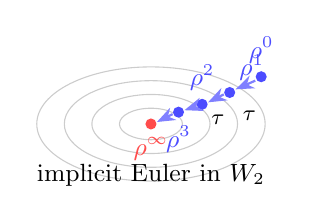
\begin{tikzpicture}[scale=0.5]
    % Energy landscape (contour)
    \foreach \r in {0.8, 1.5, 2.2, 2.9} {
        \draw[gray!40] (0,-0.5) ellipse ({\r} and {\r*0.5});
    }

    % Discrete steps
    \fill[blue!70] (2.8, 0.7) circle (4pt);
    \node[above, font=\small, blue!70] at (2.8, 0.8) {$\rho^0$};

    \fill[blue!70] (2.0, 0.3) circle (4pt);
    \node[above right, font=\small, blue!70] at (2.0, 0.35) {$\rho^1$};

    \fill[blue!70] (1.3, 0) circle (4pt);
    \node[above, font=\small, blue!70] at (1.3, 0.1) {$\rho^2$};

    \fill[blue!70] (0.7, -0.2) circle (4pt);
    \node[below, font=\small, blue!70] at (0.7, -0.3) {$\rho^3$};

    \fill[red!70] (0, -0.5) circle (4pt);
    \node[below, font=\small, red!70] at (0, -0.6) {$\rho^\infty$};

    % Arrows between steps
    \draw[-{Stealth}, thick, blue!50] (2.65, 0.6) -- (2.15, 0.38);
    \draw[-{Stealth}, thick, blue!50] (1.85, 0.25) -- (1.45, 0.05);
    \draw[-{Stealth}, thick, blue!50] (1.15, -0.05) -- (0.85, -0.15);
    \draw[-{Stealth}, thick, blue!50] (0.55, -0.25) -- (0.15, -0.45);

    % Time step annotation
    \node at (2.5, -0.3) {\footnotesize $\tau$};
    \node at (1.7, -0.4) {\footnotesize $\tau$};

    \node at (0, -1.8) {\small implicit Euler in $W_2$};
\end{tikzpicture}

\vspace{0.2cm}
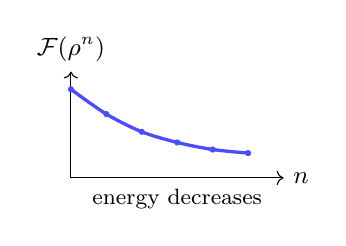
\begin{tikzpicture}[scale=0.45]
    % Energy vs iteration
    \draw[->] (0,0) -- (6,0) node[right] {\small $n$};
    \draw[->] (0,0) -- (0,3) node[above] {\small $\mathcal{F}(\rho^n)$};

    % Energy decay
    \draw[blue!70, very thick] plot[smooth] coordinates {(0,2.5) (1,1.8) (2,1.3) (3,1) (4,0.8) (5,0.7)};

    % Points
    \foreach \x/\y in {0/2.5, 1/1.8, 2/1.3, 3/1, 4/0.8, 5/0.7} {
        \fill[blue!70] (\x, \y) circle (2.5pt);
    }

    \node[font=\footnotesize] at (3, -0.6) {energy decreases};
\end{tikzpicture}
\end{center}
\end{column}
\end{columns}
\end{frame}

%==============================================================================
\section{Geometry and Curvature}
%==============================================================================

\begin{frame}{Entropy and Ricci Curvature}
\begin{columns}
\begin{column}{0.55\textwidth}
\textbf{Remarkable connection} (Lott-Villani, Sturm, 2006-2009):

\vspace{0.2cm}
On a Riemannian manifold $(M,g)$:
\[
\underbrace{E(\rho) = \int \rho \log \rho}_{\text{entropy}} \text{ is geodesically convex in } W_2
\]
\[
\Updownarrow
\]
\[
\text{Ricci curvature} \geq 0
\]

\vspace{0.2cm}
\textbf{Synthetic Ricci curvature:} For metric measure spaces $(X,d,m)$:
\[
\text{Ric} \geq K \;\Leftrightarrow\; E \text{ is } K\text{-convex along geodesics}
\]

\vspace{0.2cm}
This extends curvature bounds to \textbf{non-smooth spaces}.
\end{column}
\begin{column}{0.45\textwidth}
\begin{center}
\textbf{Geodesic Convexity}

\vspace{0.2cm}
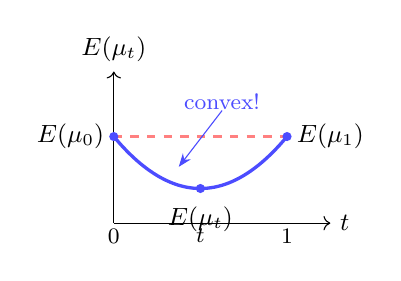
\begin{tikzpicture}[scale=0.55]
    % Convex curve
    \draw[->] (0,0) -- (5,0) node[right] {\small $t$};
    \draw[->] (0,0) -- (0,3.5) node[above] {\small $E(\mu_t)$};

    % Geodesic convexity curve
    \draw[blue!70, very thick] plot[smooth, domain=0:4] (\x, {0.3*(\x-2)^2 + 0.8});

    % Linear interpolation (dashed)
    \draw[red!50, dashed, thick] (0, 2) -- (4, 2);

    % Points
    \fill[blue!70] (0, 2) circle (3pt);
    \node[left, font=\small] at (0, 2) {$E(\mu_0)$};
    \fill[blue!70] (4, 2) circle (3pt);
    \node[right, font=\small] at (4, 2) {$E(\mu_1)$};
    \fill[blue!70] (2, 0.8) circle (3pt);
    \node[below, font=\small] at (2, 0.6) {$E(\mu_t)$};

    % Labels
    \node[font=\footnotesize] at (0, -0.3) {$0$};
    \node[font=\footnotesize] at (4, -0.3) {$1$};
    \node[font=\footnotesize] at (2, -0.3) {$t$};

    % Annotation
    \node[blue!70, font=\footnotesize] at (2.5, 2.8) {convex!};
    \draw[-{Stealth}, blue!70] (2.5, 2.6) -- (1.5, 1.3);
\end{tikzpicture}

\vspace{0.3cm}
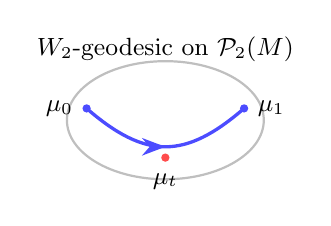
\begin{tikzpicture}[scale=0.5]
    % Geodesic on manifold
    \draw[gray!50, thick] (0,0) ellipse (2.5 and 1.5);

    % Geodesic path
    \draw[blue!70, very thick,
        decoration={markings, mark=at position 0.5 with {\arrow{Stealth}}},
        postaction={decorate}]
        (-2, 0.3) .. controls (-0.5, -1) and (0.5, -1) .. (2, 0.3);

    % Points
    \fill[blue!70] (-2, 0.3) circle (3pt);
    \node[left, font=\small] at (-2.1, 0.3) {$\mu_0$};
    \fill[red!70] (0, -0.95) circle (3pt);
    \node[below, font=\small] at (0, -1.1) {$\mu_t$};
    \fill[blue!70] (2, 0.3) circle (3pt);
    \node[right, font=\small] at (2.1, 0.3) {$\mu_1$};

    \node at (0, 1.8) {\small $W_2$-geodesic on $\mathcal{P}_2(M)$};
\end{tikzpicture}
\end{center}
\end{column}
\end{columns}
\end{frame}

%==============================================================================
\section{Applications}
%==============================================================================

\begin{frame}{Applications of Optimal Transport}
\textbf{Image Processing:}
\begin{itemize}
    \item Color transfer
    \item Shape interpolation via $W_2$ geodesics
    \item Wasserstein barycenters: $\bar\mu = \arg\min_\mu \sum_i \lambda_i W_2^2(\mu, \mu_i)$
\end{itemize}

\vspace{0.3cm}
\textbf{Machine Learning:}
\begin{itemize}
    \item Wasserstein GANs
    \item Domain adaptation
    \item Distributional distances
\end{itemize}

\vspace{0.3cm}
\textbf{Economics \& Traffic:}
\begin{itemize}
    \item Spatial economics (supply/demand allocation)
    \item Traffic congestion: $\min \int g(\rho) |v| \, dx\,dt$
    \item Branched transport: subadditive costs $m^\alpha$ ($0 < \alpha < 1$)
\end{itemize}
\end{frame}

%==============================================================================
\section{Computational Methods}
%==============================================================================

\begin{frame}{Computational Methods}
\textbf{1. Linear Programming:}
\begin{itemize}
    \item Exact for discrete measures
    \item Hungarian algorithm: $O(n^3)$
\end{itemize}

\vspace{0.3cm}
\textbf{2. Entropic Regularization} (Cuturi, 2013):
\[
\min_{\gamma \in \Pi(\mu,\nu)} \int c \, d\gamma + \underbrace{\varepsilon \int \gamma \log \gamma}_{\text{entropy penalty}}
\]

\begin{itemize}
    \item \textbf{Sinkhorn algorithm:} Iterative matrix scaling
    \item Nearly linear complexity
    \item Differentiable $\Rightarrow$ deep learning applications
\end{itemize}

\vspace{0.3cm}
\textbf{3. Semi-discrete methods:}
\begin{itemize}
    \item One continuous, one discrete measure
    \item Laguerre tessellation / power diagrams
\end{itemize}
\end{frame}

%==============================================================================
\begin{frame}{Summary}
\textbf{Theory:}
\begin{itemize}
    \item Monge (1781): Transport maps, $\min \int |T(x)-x| f(x)\,dx$
    \item Kantorovich (1942): Transport plans, linear programming
    \item Brenier (1991): $T = \nabla u$ for quadratic cost
\end{itemize}

\vspace{0.3cm}
\textbf{Geometry:}
\begin{itemize}
    \item Wasserstein distance $W_p$
    \item Geodesics, displacement convexity
    \item Gradient flows for PDEs
    \item Ricci curvature bounds
\end{itemize}

\vspace{0.3cm}
\textbf{Computation:}
\begin{itemize}
    \item Sinkhorn algorithm (entropic regularization)
    \item GPU-accelerated methods for ML
\end{itemize}
\end{frame}

\end{document}
